% Working manuscript: GluNet and CRNN reproduction on OhioT1DM.
% Class: IEEEtran (swap for the target venue's template later).
% Every \TODO marks a value that must come from a run's output CSV; nothing here is a measured result.
\documentclass[conference]{IEEEtran}
\usepackage{amsmath,booktabs,graphicx,cite}
\newcommand{\TODO}[1]{\textbf{[TODO: #1]}}
\begin{document}
\title{Reproducing GluNet and CRNN for Personalised Glucose Forecasting on OhioT1DM: Benchmarks Against Recurrent, Convolutional, Transformer and Hybrid Baselines}
\author{\IEEEauthorblockN{Sulabh Yadav}\IEEEauthorblockA{BS in Data Science and Applications, IIT Madras\\ Email: sulabhyadav176@gmail.com}}
\maketitle

\begin{abstract}
Published glucose-forecasting models are usually evaluated on different cohorts and protocols, which makes reported gains hard to compare. We reproduce two such models, a convolutional recurrent network (CRNN) and the dilated-convolution GluNet, on all 12 patients of the OhioT1DM dataset at 30- and 60-minute horizons, using the predefined training and testing partitions, a chronological validation split and a leakage-checked pipeline. We compare them on common test timestamps with last-value persistence and with GRU, LSTM, BiLSTM, TCN and Transformer baselines trained through the same pipeline, using RMSE, MAE, MARD, time lag and Clarke error grid zones. All learned models lower RMSE by roughly 12--16\% relative to persistence at both horizons, but differences among them (at most about 0.5~mg/dL at 30~min and 1~mg/dL at 60~min between the CRNN and the other well-trained models) are small relative to between-patient variability, and none is significant after Holm correction. The GluNet label transform as published clips most 30- and 60-minute glucose changes; an unclipped regression variant is better in 10/12 and 12/12 patients (planned paired comparison, uncorrected $p=0.002$ and $0.0005$). All models show long prediction lags (about 23~min at 30~min and 49~min at 60~min), and the short lags reported in the original papers are not reproduced.
\end{abstract}
\begin{IEEEkeywords}
glucose forecasting, type 1 diabetes, OhioT1DM, GluNet, CRNN, reproducibility
\end{IEEEkeywords}

\section{Introduction}
Accurate short-term glucose forecasts allow people with type~1 diabetes and automated insulin delivery systems to act before hypo- or hyperglycaemia occurs. Many forecasting models have been proposed, but they are typically trained and tested on different cohorts, input sets, splits and metrics, so published numbers are rarely comparable. Deep models such as GluNet~\cite{glunet} and the CRNN~\cite{crnn} reported strong results on simulated data and on private clinical datasets; their behaviour on a public benchmark with a fixed protocol is less clear.

This work makes three contributions. (i)~We reproduce the CRNN and GluNet on all 12 OhioT1DM patients~\cite{ohio} with a leakage-controlled pipeline and explicitly separate settings given in the papers from adaptations we had to make. (ii)~We evaluate all models on identical test timestamps against a last-value baseline, with per-patient results, paired tests and Clarke error grid analysis. (iii)~We identify where the published descriptions are ambiguous or inconsistent (residual dimensions in the CRNN, the clipping range of the GluNet label transform) and quantify their effect. The aim is a reliable benchmark on which later architectural changes can be judged.
\section{Related Work}
Classical glucose predictors include autoregressive models with exogenous inputs, latent-variable regression~\cite{lvx} and support vector regression~\cite{svr}. Neural networks for glucose prediction date back at least to~\cite{nnpg}, which used small feed-forward networks on glucose data. GluNet~\cite{glunet} adapts the gated, dilated causal convolutions of WaveNet~\cite{wavenet} to forecast the change in glucose as a classification over quantised bins, and reports results on simulated data, a private clinical cohort and six OhioT1DM subjects~\cite{ohio}. The CRNN~\cite{crnn} stacks convolution and pooling layers in front of a modified LSTM~\cite{lstm} that predicts the glucose change and adds it back to the current value, and is evaluated on simulated data and a private clinical cohort. Both papers compare against ARX, LVX, SVR and a neural-network baseline and report RMSE, MARD and a prediction-lag measure based on cross-correlation. Clinical accuracy is commonly assessed with the Clarke error grid~\cite{clarke}. We do not claim novelty in the models; the contribution is a matched-protocol comparison.
\section{Materials and Methods}
\subsection{Dataset}
OhioT1DM 2018 (patients 559, 563, 570, 575, 588, 591) and 2020 (540, 544, 552, 567, 584, 596) releases, 12 patients, predefined training/testing partitions. The published GluNet OhioT1DM evaluation used six subjects, so 12-patient results are an extension, not an exact replication.

\subsection{Preprocessing and Leakage Control}
Data are on a 5-minute grid. Our pipeline does not interpolate: a window is kept only if all of its input rows lie in one continuous segment (a new segment starts where the timestamp gap exceeds the repository's threshold) and the row exactly $h$ minutes after the window end exists in the same segment; no window or target crosses a segment or split boundary, so no interpolated value can reach scoring (stricter than the papers, which interpolate gaps up to one hour and exclude those points). The chronological validation split is the final 15\% of rows of each patient's training partition, taken before windowing, with an explicit check that no training target reaches the validation period. In the primary CRNN configuration inputs are standardised per channel using statistics of the training windows only; targets and the recovery step stay in mg/dL. No Gaussian smoothing is applied, because the CRNN paper does not give a filter width (and a symmetric filter would use samples after the forecast origin); this is a deviation. GluNet uses its own gap-safe pipeline with 16-step windows and the same split principle.

\section{GluNet and CRNN Architectures}
\subsection{GluNet}
The paper specifies five layers (32, 32, 32, 64, 64 units), dilations $\{1,2,4,8\}$, gated activations with residual and skip connections, a 16-step window, inputs of glucose, meals, insulin and time stamps, and a 256-class softmax over the glucose change $\Delta G=G_{t+w}-G_t$ quantised at 0.1~mg/dL, clipped outside about $[-12.75,12.85]$~mg/dL (Eq.~(4)); the absolute value is recovered as $G_t+\widehat{\Delta G}$. Padding, the optimiser, skip-connection details and the class-to-glucose decoding are not specified, so our implementation (an input projection followed by four gated blocks) is a documented interpretation, and both a probability-weighted and an argmax decoder were evaluated (results shown use the probability-weighted one). Because the clipping removes most 30- and 60-minute changes (see Limitations), we also report GluNet-regression, an adaptation that regresses the unclipped change with the same network. The optional $P_i$ and $R_a$ inputs are not implemented and are left to future work.

\subsection{CRNN}
Inputs: glucose, carbohydrates, insulin; 24-step (2~h) window; target is the glucose change $x(t+w)-x(t)$, recovered by adding $x(t)$; mean-absolute-error loss; RMSprop. Following the paper's Table~V: three 1$\times$4 convolutions with 8, 16 and 32 channels, each followed by max-pooling of size 2 (24$\to$12$\to$6$\to$3 steps), an LSTM with 64 cells whose input is 32-dimensional (24{,}832 parameters, single bias), dense layers of 256 and 32 units and a linear output; batch size 128 in the paper's table. The modified cell outputs $y_t=o_t\odot\tanh(c_t)+x_t$. In the paper $x_t$ is 32-dimensional while $h_t$ has 64 units, so the residual addition is dimensionally inconsistent as written. We add a learned bias-free $32\to64$ projection (2{,}048 parameters), an \emph{adaptation}. Our LSTM has 27{,}136 parameters, i.e.\ 24{,}832 $+$ 256 (PyTorch's second bias vector) $+$ 2{,}048 (projection), so the remaining difference from Table~V is fully accounted for. The paper does not specify the Gaussian-filter width, dropout rate or padding.

\section{Experimental Setup and Evaluation Metrics}
Patient-specific models are trained for each horizon. The 30- and 60-minute horizons are complete; 15, 90 and 120~min are pending. Every patient/horizon uses seed 42; training ran on an Apple MacBook Air (MPS). CRNN settings: RMSprop (learning rate $10^{-3}$), mean-absolute-error loss on the glucose change, batch 128, dropout 0.2, up to 50 epochs with early stopping (patience 7) on validation loss; the best-validation checkpoint is evaluated once on the test partition. Metrics: RMSE, MAE, MARD, time lag and Clarke zones A--E. The lag $\tau$ is the shift (5-min grid) maximising the cross-correlation between the prediction and the reference; positive means the prediction trails the reference, so last-value persistence gives exactly the horizon (30 and 60~min), which we use as a check of the implementation, together with the repository's unit tests. All models are scored on the same eligible test timestamps.

\begin{table*}[t]\centering\caption{Test-partition results on OhioT1DM, 12 patients, mean $\pm$ SD across patients, on the common eligible test timestamps of all models. CRNN$^{*}$: primary configuration (batch 128, inputs standardised with training statistics); CRNN$^{\dagger}$: batch-256, unstandardised ablation. GluNet-literal: the paper's Eq.~(4) label transform (256 classes, clipped at about $\pm$12.8~mg/dL; 48\% and 67\% of test windows clipped at 30 and 60~min), probability-weighted decoder; GluNet-regression: adaptation regressing the unclipped change. GRU, LSTM, BiLSTM, TCN and Transformer are small untuned models (15--39\,k parameters) trained with the CRNN recipe and the same change-and-recover target. Source: \texttt{output/benchmark/summary\_12.csv}.}
\small\begin{tabular}{llccccc}\toprule
Hor. & Model & RMSE & MAE & MARD (\%) & Lag (min) & CEG A (\%)\\\midrule
30 & CRNN$^{*}$ & 19.86$\pm$2.40 & 13.94$\pm$1.63 & 9.39$\pm$1.69 & 23.3$\pm$3.3 & 88.6$\pm$4.0\\
30 & CRNN$^{\dagger}$ & 19.51$\pm$2.33 & 13.62$\pm$1.58 & 9.10$\pm$1.55 & 23.3$\pm$3.3 & 89.4$\pm$3.5\\
30 & GluNet-regression & 19.65$\pm$2.23 & 13.95$\pm$1.42 & 9.39$\pm$1.58 & 23.3$\pm$3.3 & 88.9$\pm$4.0\\
30 & GluNet-literal & 20.74$\pm$2.74 & 14.71$\pm$2.00 & 9.91$\pm$2.03 & 27.9$\pm$2.6 & 87.3$\pm$5.2\\
30 & GRU & 19.69$\pm$2.42 & 13.86$\pm$1.69 & 9.33$\pm$1.77 & 22.5$\pm$4.5 & 88.8$\pm$4.2\\
30 & LSTM & 20.30$\pm$2.79 & 14.47$\pm$2.01 & 9.75$\pm$1.98 & 24.2$\pm$4.2 & 87.7$\pm$4.7\\
30 & BiLSTM & 20.04$\pm$2.86 & 14.25$\pm$1.98 & 9.57$\pm$1.86 & 25.0$\pm$3.0 & 88.1$\pm$4.7\\
30 & TCN & 19.54$\pm$2.18 & 13.71$\pm$1.51 & 9.20$\pm$1.58 & 22.5$\pm$3.4 & 89.0$\pm$3.5\\
30 & Transformer & 20.03$\pm$2.61 & 14.07$\pm$1.82 & 9.47$\pm$1.84 & 24.2$\pm$3.6 & 88.3$\pm$4.4\\
30 & Persistence & 23.14$\pm$2.87 & 16.79$\pm$2.05 & 11.29$\pm$2.08 & 30.0$\pm$0.0 & 83.6$\pm$5.9\\
\midrule
60 & CRNN$^{*}$ & 32.72$\pm$4.35 & 23.87$\pm$3.10 & 16.31$\pm$3.09 & 49.2$\pm$7.0 & 71.7$\pm$7.9\\
60 & CRNN$^{\dagger}$ & 32.54$\pm$3.48 & 23.70$\pm$2.56 & 15.91$\pm$2.86 & 49.2$\pm$8.8 & 72.0$\pm$8.0\\
60 & GluNet-regression & 32.68$\pm$3.96 & 24.12$\pm$3.08 & 16.56$\pm$3.25 & 50.0$\pm$7.4 & 70.2$\pm$9.1\\
60 & GluNet-literal & 35.05$\pm$4.32 & 25.61$\pm$3.17 & 17.33$\pm$3.26 & 58.8$\pm$2.3 & 68.6$\pm$7.7\\
60 & GRU & 32.39$\pm$4.36 & 23.82$\pm$3.29 & 16.12$\pm$3.38 & 49.6$\pm$8.7 & 71.6$\pm$9.1\\
60 & LSTM & 33.26$\pm$4.24 & 24.51$\pm$3.25 & 16.53$\pm$3.25 & 51.3$\pm$7.4 & 70.5$\pm$9.2\\
60 & BiLSTM & 32.63$\pm$4.25 & 24.06$\pm$3.25 & 16.34$\pm$3.38 & 50.4$\pm$7.8 & 71.2$\pm$8.7\\
60 & TCN & 32.31$\pm$3.88 & 23.69$\pm$3.09 & 16.13$\pm$3.40 & 48.8$\pm$8.0 & 71.6$\pm$8.6\\
60 & Transformer & 33.16$\pm$4.14 & 24.10$\pm$3.23 & 16.39$\pm$3.29 & 49.6$\pm$8.4 & 71.2$\pm$8.5\\
60 & Persistence & 37.99$\pm$4.66 & 28.16$\pm$3.40 & 19.09$\pm$3.50 & 60.0$\pm$0.0 & 65.0$\pm$8.3\\
\bottomrule
\end{tabular}\end{table*}
\begin{table}[t]\centering\caption{Published GluNet (Li et al., Table~IV, 6 OhioT1DM 2018 subjects, 5-model comparison, its own protocol) vs.\ our CRNN on the same six subjects (559, 563, 570, 575, 588, 591). Not a like-for-like comparison: different model, windows and validation split. Our SDs are in \texttt{output/benchmark/summary\_6.csv}.}
\small\begin{tabular}{llccc}\toprule
Hor. & Source & RMSE & MARD (\%) & Lag (min)\\\midrule
30 & GluNet, published & 19.28$\pm$2.76 & 8.73$\pm$1.78 & 8.03$\pm$4.07\\
30 & CRNN$^{*}$, ours (6 subj.) & 19.86 & 8.92 & 25.0\\
30 & GluNet-regression, ours (6 subj.) & 19.65 & 8.99 & 25.0\\
60 & GluNet, published & 31.83$\pm$3.49 & 16.11$\pm$4.49 & 17.78$\pm$8.00\\
60 & CRNN$^{*}$, ours (6 subj.) & 32.04 & 15.44 & 51.7\\
60 & GluNet-regression, ours (6 subj.) & 31.82 & 15.61 & 53.3\\\bottomrule
\end{tabular}\end{table}
\begin{table}[t]\centering\caption{Published CRNN (Li et al., Tables~II--IV): 10 clinical adults of the Imperial/St Mary's study, 6 months of data split 50/50, own protocol, \emph{not} OhioT1DM. Shown only for context.}
\small\begin{tabular}{lccc}\toprule
Hor. & RMSE & MARD (\%) & PH$_{\rm eff}$ (min)\\\midrule
30 & 21.07$\pm$2.35 & 11.61$\pm$2.18 & 19.3$\pm$3.1\\
60 & 33.27$\pm$4.79 & 19.01$\pm$4.46 & 29.3$\pm$9.4\\\bottomrule
\end{tabular}\end{table}
\paragraph{Time lag.} The published GluNet reports lags of 8.0 and 17.8~min on OhioT1DM (30/60~min). Our models do not reproduce this: pooled cross-correlation gives 23.3 and 49.2~min (CRNN) and 23.3 and 50.0~min (GluNet-regression); a per-three-day-period version following the paper's description gives 22.5/46.9 and 23.7/48.1~min, while last-value persistence gives exactly 30 and 60~min, validating the implementation. The metric definition therefore does not explain the gap; we make no claim about its cause.
\paragraph{Discussion.} All models land in a narrow band: at 30~min RMSE 19.5--20.3~mg/dL for the learned models (persistence 23.1) and at 60~min 32.3--33.3 (persistence 38.0), except GluNet-literal (20.7 and 35.1). On the six patients used in the GluNet paper, GluNet-regression gives 19.65 and 31.82~mg/dL against the published 19.28 and 31.83; the CRNN was published on a different, private cohort (21.07 and 33.27). These comparisons are indicative only, because cohorts, splits, windows and training data differ; possible reasons for the remaining differences (cohort size, preprocessing, input set, evaluation protocol, our stricter gap handling) were not tested. The weak spot common to all models is lag, not magnitude of error.

\IfFileExists{tables/patientwise_RMSE_30.tex}{\begin{table*}[t]\centering
\caption{Patient-wise RMSE (mg/dL) at 30~min on common test windows; best per patient in bold. CRNN: primary configuration; CRNN-256: batch-256 ablation; GN-reg/GN-lit: GluNet regression/literal. Source: \texttt{output/benchmark/patientwise.csv}.}
\scriptsize\setlength{\tabcolsep}{3pt}
\begin{tabular}{lrcccccccccc}\toprule
Patient & $n$ & CRNN & CRNN-256 & GN-reg & GN-lit & GRU & LSTM & BiLSTM & TCN & Trans. & Persist.\\\midrule
540 & 2434 & 22.38 & \textbf{21.25} & 22.08 & 25.42 & 21.69 & 24.04 & 24.56 & 21.86 & 23.37 & 28.60\\
544 & 2484 & 16.95 & 17.14 & \textbf{16.31} & 18.07 & 17.19 & 17.14 & 16.81 & 17.08 & 17.48 & 21.90\\
552 & 1882 & 18.74 & \textbf{17.87} & 18.72 & 19.96 & 17.91 & 19.16 & 18.52 & 18.15 & 18.87 & 21.37\\
559 & 2166 & 19.71 & \textbf{18.46} & 19.70 & 20.09 & 19.36 & 19.30 & 19.05 & 19.09 & 19.35 & 22.81\\
563 & 2454 & 20.68 & 18.73 & \textbf{18.61} & 19.02 & 19.55 & 20.50 & 19.83 & 19.36 & 19.77 & 20.89\\
567 & 1866 & 22.69 & 21.60 & 21.82 & 24.52 & 22.82 & 24.14 & 23.52 & \textbf{21.52} & 22.90 & 27.67\\
570 & 2455 & 16.24 & \textbf{15.97} & 16.42 & 16.41 & 16.46 & 16.28 & 16.54 & 16.34 & 16.09 & 18.52\\
575 & 2286 & 22.79 & 22.74 & 22.54 & 22.51 & 22.84 & 23.05 & 22.77 & \textbf{22.48} & 22.84 & 24.46\\
584 & 2201 & 21.52 & \textbf{20.77} & 21.51 & 22.48 & 21.38 & 21.64 & 21.26 & 21.07 & 21.52 & 24.26\\
588 & 2704 & \textbf{18.20} & 21.04 & 18.99 & 19.61 & 18.54 & 18.85 & 18.63 & 19.12 & 18.63 & 21.86\\
591 & 2616 & \textbf{21.56} & 22.03 & 21.64 & 22.55 & 22.16 & 22.60 & 22.68 & 21.74 & 22.85 & 24.11\\
596 & 2540 & 16.90 & 16.53 & 17.52 & 18.28 & 16.44 & 16.90 & \textbf{16.36} & 16.63 & 16.67 & 21.28\\
\midrule
Mean$\pm$SD & & 19.86$\pm$2.40 & 19.51$\pm$2.33 & 19.65$\pm$2.23 & 20.74$\pm$2.74 & 19.69$\pm$2.42 & 20.30$\pm$2.79 & 20.04$\pm$2.86 & 19.54$\pm$2.18 & 20.03$\pm$2.61 & 23.14$\pm$2.87\\
\bottomrule
\end{tabular}\end{table*}
}{}
\IfFileExists{tables/patientwise_RMSE_60.tex}{\begin{table*}[t]\centering
\caption{Patient-wise RMSE (mg/dL) at 60~min on common test windows; best per patient in bold. CRNN: primary configuration; CRNN-256: batch-256 ablation; GN-reg/GN-lit: GluNet regression/literal. Source: \texttt{output/benchmark/patientwise.csv}.}
\scriptsize\setlength{\tabcolsep}{3pt}
\begin{tabular}{lrcccccccccc}\toprule
Patient & $n$ & CRNN & CRNN-256 & GN-reg & GN-lit & GRU & LSTM & BiLSTM & TCN & Trans. & Persist.\\\midrule
540 & 2182 & 41.27 & \textbf{39.33} & 39.54 & 43.84 & 39.88 & 41.46 & 40.64 & 39.74 & 40.08 & 47.47\\
544 & 2436 & 28.07 & 28.36 & 27.60 & 32.39 & 28.00 & 27.65 & \textbf{27.51} & 28.02 & 29.22 & 36.91\\
552 & 1661 & \textbf{30.53} & 33.88 & 31.10 & 33.13 & 32.17 & 33.00 & 30.56 & 31.44 & 32.45 & 35.02\\
559 & 2094 & 31.04 & 31.02 & 32.42 & 35.24 & \textbf{30.77} & 33.18 & 32.10 & 32.52 & 33.41 & 38.35\\
563 & 2430 & 35.22 & 31.00 & \textbf{30.75} & 32.00 & 32.57 & 31.83 & 31.41 & 31.23 & 31.86 & 34.21\\
567 & 1644 & 38.25 & \textbf{36.95} & 38.42 & 42.06 & 40.14 & 39.86 & 39.13 & 37.66 & 39.73 & 46.02\\
570 & 2395 & \textbf{26.51} & 26.63 & 27.37 & 28.61 & 27.04 & 27.72 & 27.54 & 27.41 & 26.98 & 31.02\\
575 & 2226 & 34.49 & 34.52 & 35.26 & 35.27 & 33.63 & 34.40 & 34.55 & \textbf{33.63} & 34.22 & 37.98\\
584 & 2105 & 34.37 & \textbf{32.61} & 35.76 & 37.27 & 33.48 & 33.60 & 34.55 & 34.38 & 34.95 & 39.25\\
588 & 2686 & 31.78 & 32.58 & 31.75 & 33.07 & 30.41 & 31.03 & 30.65 & \textbf{30.26} & 31.50 & 35.76\\
591 & 2592 & \textbf{33.19} & 33.20 & 33.35 & 35.62 & 34.01 & 35.54 & 34.65 & 34.01 & 35.69 & 38.02\\
596 & 2498 & 27.87 & 30.42 & 28.85 & 32.15 & \textbf{26.62} & 29.88 & 28.27 & 27.43 & 27.84 & 35.85\\
\midrule
Mean$\pm$SD & & 32.72$\pm$4.35 & 32.54$\pm$3.48 & 32.68$\pm$3.96 & 35.05$\pm$4.32 & 32.39$\pm$4.36 & 33.26$\pm$4.24 & 32.63$\pm$4.25 & 32.31$\pm$3.88 & 33.16$\pm$4.14 & 37.99$\pm$4.66\\
\bottomrule
\end{tabular}\end{table*}
}{}
\IfFileExists{tables/patientwise_MARD_30.tex}{\begin{table*}[t]\centering
\caption{Patient-wise MARD (\%) at 30~min on common test windows; best per patient in bold. CRNN: primary configuration; CRNN-256: batch-256 ablation; GN-reg/GN-lit: GluNet regression/literal. Source: \texttt{output/benchmark/patientwise.csv}.}
\scriptsize\setlength{\tabcolsep}{3pt}
\begin{tabular}{lrcccccccccc}\toprule
Patient & $n$ & CRNN & CRNN-256 & GN-reg & GN-lit & GRU & LSTM & BiLSTM & TCN & Trans. & Persist.\\\midrule
540 & 2434 & 10.90 & \textbf{10.35} & 11.15 & 12.64 & 10.99 & 11.77 & 11.92 & 10.63 & 11.34 & 14.70\\
544 & 2484 & 7.93 & 7.89 & \textbf{7.80} & 8.35 & 7.98 & 7.93 & 7.97 & 8.05 & 8.02 & 10.71\\
552 & 1882 & 10.35 & 10.07 & 10.05 & 11.16 & \textbf{9.74} & 10.23 & 10.16 & 9.86 & 10.19 & 11.60\\
559 & 2166 & 8.68 & \textbf{7.76} & 8.53 & 8.64 & 8.34 & 8.47 & 8.56 & 8.33 & 8.53 & 10.22\\
563 & 2454 & 8.87 & \textbf{8.10} & 8.33 & 8.53 & 8.33 & 9.00 & 8.52 & 8.33 & 8.58 & 9.68\\
567 & 1866 & 10.74 & \textbf{9.97} & 10.61 & 11.90 & 10.87 & 12.02 & 11.52 & 10.17 & 10.99 & 13.65\\
570 & 2455 & \textbf{5.81} & 5.97 & 6.32 & 6.12 & 5.98 & 6.06 & 6.24 & 5.90 & 5.85 & 7.17\\
575 & 2286 & 10.28 & \textbf{10.25} & 10.86 & 11.02 & 10.33 & 11.12 & 10.69 & 10.27 & 10.72 & 12.54\\
584 & 2201 & 10.49 & \textbf{9.71} & 10.02 & 10.32 & 10.28 & 10.61 & 9.99 & 10.03 & 10.27 & 11.02\\
588 & 2704 & \textbf{7.99} & 9.11 & 8.29 & 8.26 & 8.11 & 8.27 & 8.24 & 8.46 & 8.06 & 9.60\\
591 & 2616 & 11.89 & 11.74 & \textbf{11.60} & 12.64 & 12.47 & 12.74 & 12.49 & 11.91 & 12.49 & 13.47\\
596 & 2540 & 8.70 & \textbf{8.36} & 9.18 & 9.29 & 8.49 & 8.78 & 8.57 & 8.50 & 8.59 & 11.11\\
\midrule
Mean$\pm$SD & & 9.39$\pm$1.69 & 9.10$\pm$1.55 & 9.39$\pm$1.58 & 9.91$\pm$2.03 & 9.33$\pm$1.77 & 9.75$\pm$1.98 & 9.57$\pm$1.86 & 9.20$\pm$1.58 & 9.47$\pm$1.84 & 11.29$\pm$2.08\\
\bottomrule
\end{tabular}\end{table*}
}{}
\IfFileExists{tables/patientwise_MARD_60.tex}{\begin{table*}[t]\centering
\caption{Patient-wise MARD (\%) at 60~min on common test windows; best per patient in bold. CRNN: primary configuration; CRNN-256: batch-256 ablation; GN-reg/GN-lit: GluNet regression/literal. Source: \texttt{output/benchmark/patientwise.csv}.}
\scriptsize\setlength{\tabcolsep}{3pt}
\begin{tabular}{lrcccccccccc}\toprule
Patient & $n$ & CRNN & CRNN-256 & GN-reg & GN-lit & GRU & LSTM & BiLSTM & TCN & Trans. & Persist.\\\midrule
540 & 2182 & 19.76 & \textbf{18.80} & 20.83 & 22.55 & 19.36 & 20.30 & 20.95 & 20.14 & 19.09 & 25.23\\
544 & 2436 & 13.00 & \textbf{12.61} & 13.26 & 15.46 & 13.37 & 13.24 & 13.15 & 13.17 & 13.32 & 18.28\\
552 & 1661 & 17.52 & 19.01 & 17.63 & 18.33 & 18.16 & 18.62 & \textbf{17.18} & 18.54 & 17.86 & 19.52\\
559 & 2094 & 15.79 & \textbf{13.61} & 15.61 & 15.90 & 14.34 & 15.07 & 14.06 & 14.01 & 17.14 & 17.71\\
563 & 2430 & 14.72 & 14.39 & \textbf{13.68} & 14.71 & 13.95 & 14.04 & 13.97 & 13.80 & 13.75 & 16.21\\
567 & 1644 & 19.61 & \textbf{18.15} & 20.90 & 21.26 & 21.19 & 20.92 & 20.13 & 18.84 & 20.93 & 23.60\\
570 & 2395 & \textbf{10.20} & 10.76 & 11.11 & 11.48 & 10.63 & 10.98 & 11.01 & 10.39 & 10.35 & 12.71\\
575 & 2226 & 18.86 & 18.25 & 18.72 & 18.85 & \textbf{17.42} & 18.97 & 19.03 & 19.68 & 18.25 & 20.90\\
584 & 2105 & 17.92 & \textbf{15.48} & 17.19 & 16.99 & 16.11 & 16.23 & 16.12 & 17.44 & 17.04 & 17.71\\
588 & 2686 & 13.42 & 14.60 & 14.03 & 14.37 & \textbf{13.27} & 13.68 & 13.52 & 13.31 & 13.48 & 15.99\\
591 & 2592 & \textbf{19.62} & 19.74 & 20.49 & 21.23 & 21.30 & 20.25 & 21.26 & 20.45 & 20.86 & 22.25\\
596 & 2498 & 15.28 & 15.56 & 15.32 & 16.87 & 14.34 & 16.03 & 15.66 & \textbf{13.80} & 14.64 & 19.02\\
\midrule
Mean$\pm$SD & & 16.31$\pm$3.09 & 15.91$\pm$2.86 & 16.56$\pm$3.25 & 17.33$\pm$3.26 & 16.12$\pm$3.38 & 16.53$\pm$3.25 & 16.34$\pm$3.38 & 16.13$\pm$3.40 & 16.39$\pm$3.29 & 19.09$\pm$3.50\\
\bottomrule
\end{tabular}\end{table*}
}{}
\IfFileExists{figures/rmse_by_patient.pdf}{\begin{figure}[t]\centering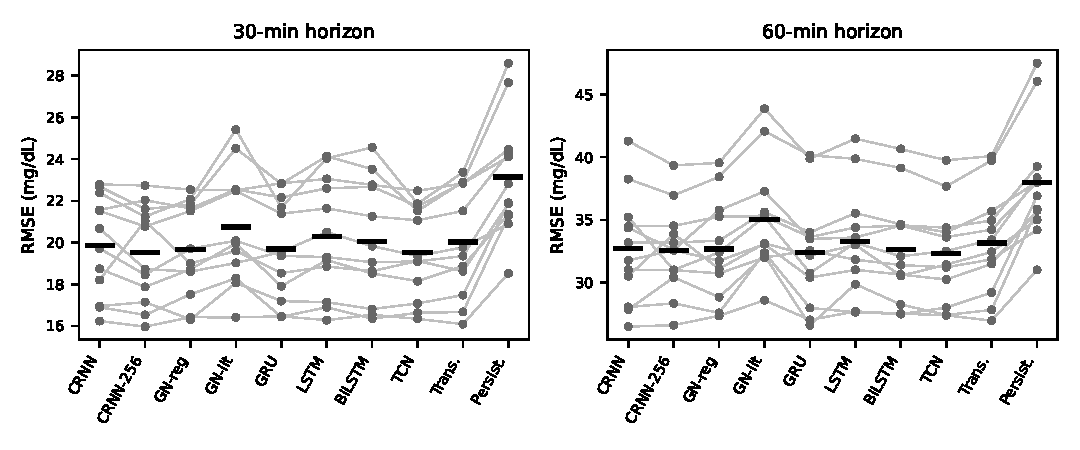
\includegraphics[width=\columnwidth]{figures/rmse_by_patient.pdf}\caption{Per-patient RMSE for every model (grey lines join the same patient; black bar: mean). Source: \texttt{output/benchmark/patientwise.csv}.}\end{figure}}{}
\TODO{Extended horizons 15/90/120~min; architecture diagrams. Patient-wise tables and the figure appear after running \texttt{experiments/make\_report\_assets.py}.}

\section{Statistical and Clinical Evaluation}
Statistical comparisons use per-patient RMSE, with the patient as the unit ($n=12$). Each model is compared with the primary CRNN by a two-sided Wilcoxon signed-rank test; $p$-values are Holm-adjusted~\cite{holm} within each horizon over the nine comparisons (eight models and persistence). With $n=12$ the smallest attainable two-sided exact $p$ is $0.0005$.

All learned models have lower RMSE than last-value persistence; for the primary CRNN the difference is significant at both horizons (CRNN better in 12/12 patients at 30~min, adjusted $p=0.0044$; 11/12 at 60~min, adjusted $p=0.0088$). Against the other learned models no difference from the CRNN survives correction (30~min: smallest adjusted $p=0.27$, GluNet-literal and LSTM; 60~min: smallest adjusted $p=0.098$, GluNet-literal). The CRNN, GRU, TCN and GluNet-regression are within about 0.3~mg/dL RMSE of each other at 30~min, and TCN, GRU, CRNN and BiLSTM within about 0.5~mg/dL at 60~min, well inside the between-patient SD of 2--4~mg/dL; with a single training seed we therefore do not rank them. The effect of the label-transform clipping was a planned contrast: GluNet-regression has lower RMSE than GluNet-literal in 10/12 patients at 30~min (mean difference 1.09~mg/dL, uncorrected $p=0.0024$) and in 12/12 at 60~min (2.37~mg/dL, $p=0.0005$).

Clinically, 87.3--89.4\% (30~min) and 68.6--72.0\% (60~min) of predictions of the learned models fall in Clarke zone~A, against 83.6\% and 65.0\% for persistence; zones~A+B exceed 99\% at 30~min and are about 96\% at 60~min for all models, including persistence. At 60~min the learned models place somewhat more predictions in zone~D (2.8--3.6\%, GluNet-literal 2.6\%) than persistence (2.5\%). We did not test this difference and report it as an observation: lower RMSE did not translate into fewer predictions in the dangerous zones. Mean time lag is 22.5--25.0~min at 30~min (GluNet-literal 27.9) and 48.8--51.3~min at 60~min (GluNet-literal 58.8), i.e.\ an effective horizon of only 5--7.5 and 9--11~min, versus lags of 8.0 and 17.8~min reported for GluNet on OhioT1DM~\cite{glunet}. A per-period lag computation following the paper's description gives similar values, and the lag of last-value persistence is exactly 30 and 60~min, which validates the implementation.
\section{Limitations}
Raw OhioT1DM data cannot be redistributed. Results use a single training seed (42); the five baselines share one recipe and are not tuned individually on Apple MPS hardware; we did not average over seeds. Our CRNN pipeline applies no Gaussian smoothing, because the paper gives no filter width, and does not interpolate gaps (windows with missing timestamps are dropped), which is stricter than the paper's protocol; inputs are standardised with training statistics only, which the paper does not describe. The CRNN's residual connection needed an added projection because the paper's dimensions are inconsistent. Validation uses the final 15\% of each patient's training partition, which for some patients behaves differently from the rest and led to early best epochs. Several architectural details are not fully specified in the papers (padding, residual dimension handling, timestamp encoding, some hyperparameters) and are marked as adaptations. The GluNet label transform as published clips most 30- and 60-minute glucose changes into the end classes, so a paper-literal implementation is compared with documented adapted variants. Results are not clinically validated, and numbers on this cohort are not expected to match the published ones.

\section{Conclusion and Future Work}
On OhioT1DM, the CRNN, GluNet-regression, GRU, LSTM, BiLSTM, TCN and Transformer all reduce RMSE by roughly 12--16\% against last-value persistence at 30 and 60 minutes, but they are statistically indistinguishable from one another with 12 patients and one seed, and their prediction lag remains close to that of persistence. The choice among these architecture families therefore matters little on this data. The GluNet label transform as published (256 classes clipped at about $\pm$12.8~mg/dL) discards most of the signal at these horizons, and the unclipped variant is better in a planned paired comparison. Before developing a new hybrid architecture, the main open gap is the long lag; future work will (i)~repeat the experiments over several seeds, (ii)~extend to 15-, 90- and 120-minute horizons, (iii)~test whether a causal input smoothing step or a lag-aware loss changes lag, and (iv)~evaluate the physiologically derived $P_i$ and $R_a$ inputs for GluNet.
\begin{thebibliography}{1}
\bibitem{glunet} K. Li \emph{et al.}, ``GluNet: A deep learning framework for accurate glucose forecasting,'' \emph{IEEE J. Biomed. Health Inform.}, 2020.
\bibitem{crnn} K. Li \emph{et al.}, ``Convolutional recurrent neural networks for glucose prediction,'' \emph{IEEE J. Biomed. Health Inform.}, 2020.
\bibitem{ohio} C. Marling and R. Bunescu, ``The OhioT1DM dataset for blood glucose level prediction,'' 2018/2020 releases. \TODO{complete citation}
\bibitem{clarke} W. L. Clarke \emph{et al.}, ``Evaluating clinical accuracy of systems for self-monitoring of blood glucose,'' \emph{Diabetes Care}, vol. 10, no. 5, pp. 622--628, 1987.
\bibitem{holm} S. Holm, ``A simple sequentially rejective multiple test procedure,'' \emph{Scand. J. Statist.}, vol. 6, no. 2, pp. 65--70, 1979.
\bibitem{nnpg} C. P\'erez-Gand\'ia \emph{et al.}, ``Artificial neural network algorithm for online glucose prediction from continuous glucose monitoring,'' \emph{Diabetes Technol. Ther.}, vol. 12, no. 1, pp. 81--88, 2010.
\bibitem{svr} E. I. Georga \emph{et al.}, ``Multivariate prediction of subcutaneous glucose concentration in type 1 diabetes patients based on support vector regression,'' \emph{IEEE J. Biomed. Health Inform.}, vol. 17, no. 1, pp. 71--81, 2013.
\bibitem{lvx} C. Zhao \emph{et al.}, ``Predicting subcutaneous glucose concentration using a latent-variable-based statistical method for type 1 diabetes mellitus,'' \emph{J. Diabetes Sci. Technol.}, vol. 6, no. 3, pp. 617--633, 2012.
\bibitem{wavenet} A. van den Oord \emph{et al.}, ``WaveNet: A generative model for raw audio,'' 2016, arXiv:1609.03499.
\bibitem{lstm} S. Hochreiter and J. Schmidhuber, ``Long short-term memory,'' \emph{Neural Comput.}, vol. 9, no. 8, pp. 1735--1780, 1997.
\end{thebibliography}
\end{document}
